\section{Area of Study}
	This study will be conducted over Metro Manila, Philippines.
	Metro Manila, formally known as the National Capital Region, is the capital region of the Philippines.
	The region has a land area of 636 square kilometers	and has a population of 13 million people (\cite{PSA2021}).
	It is composed of one municipality: Pateros, and sixteen cities:
		Caloocan,
		Las Pinas,
		Makati,
		Malabon,
		Mandaluyong,
		Manila,
		Marikina,
		Muntinlupa,
		Navotas,
		Paranaque,
		Pasay,
		Pasig,
		Quezon City,
		San Juan,
		Taguig, and
		Valenzuela.
	A map of Metro Manila is seen in Figure \ref{fig:map-of-metro-manila}.
	
	\begin{figure}
		\centering
		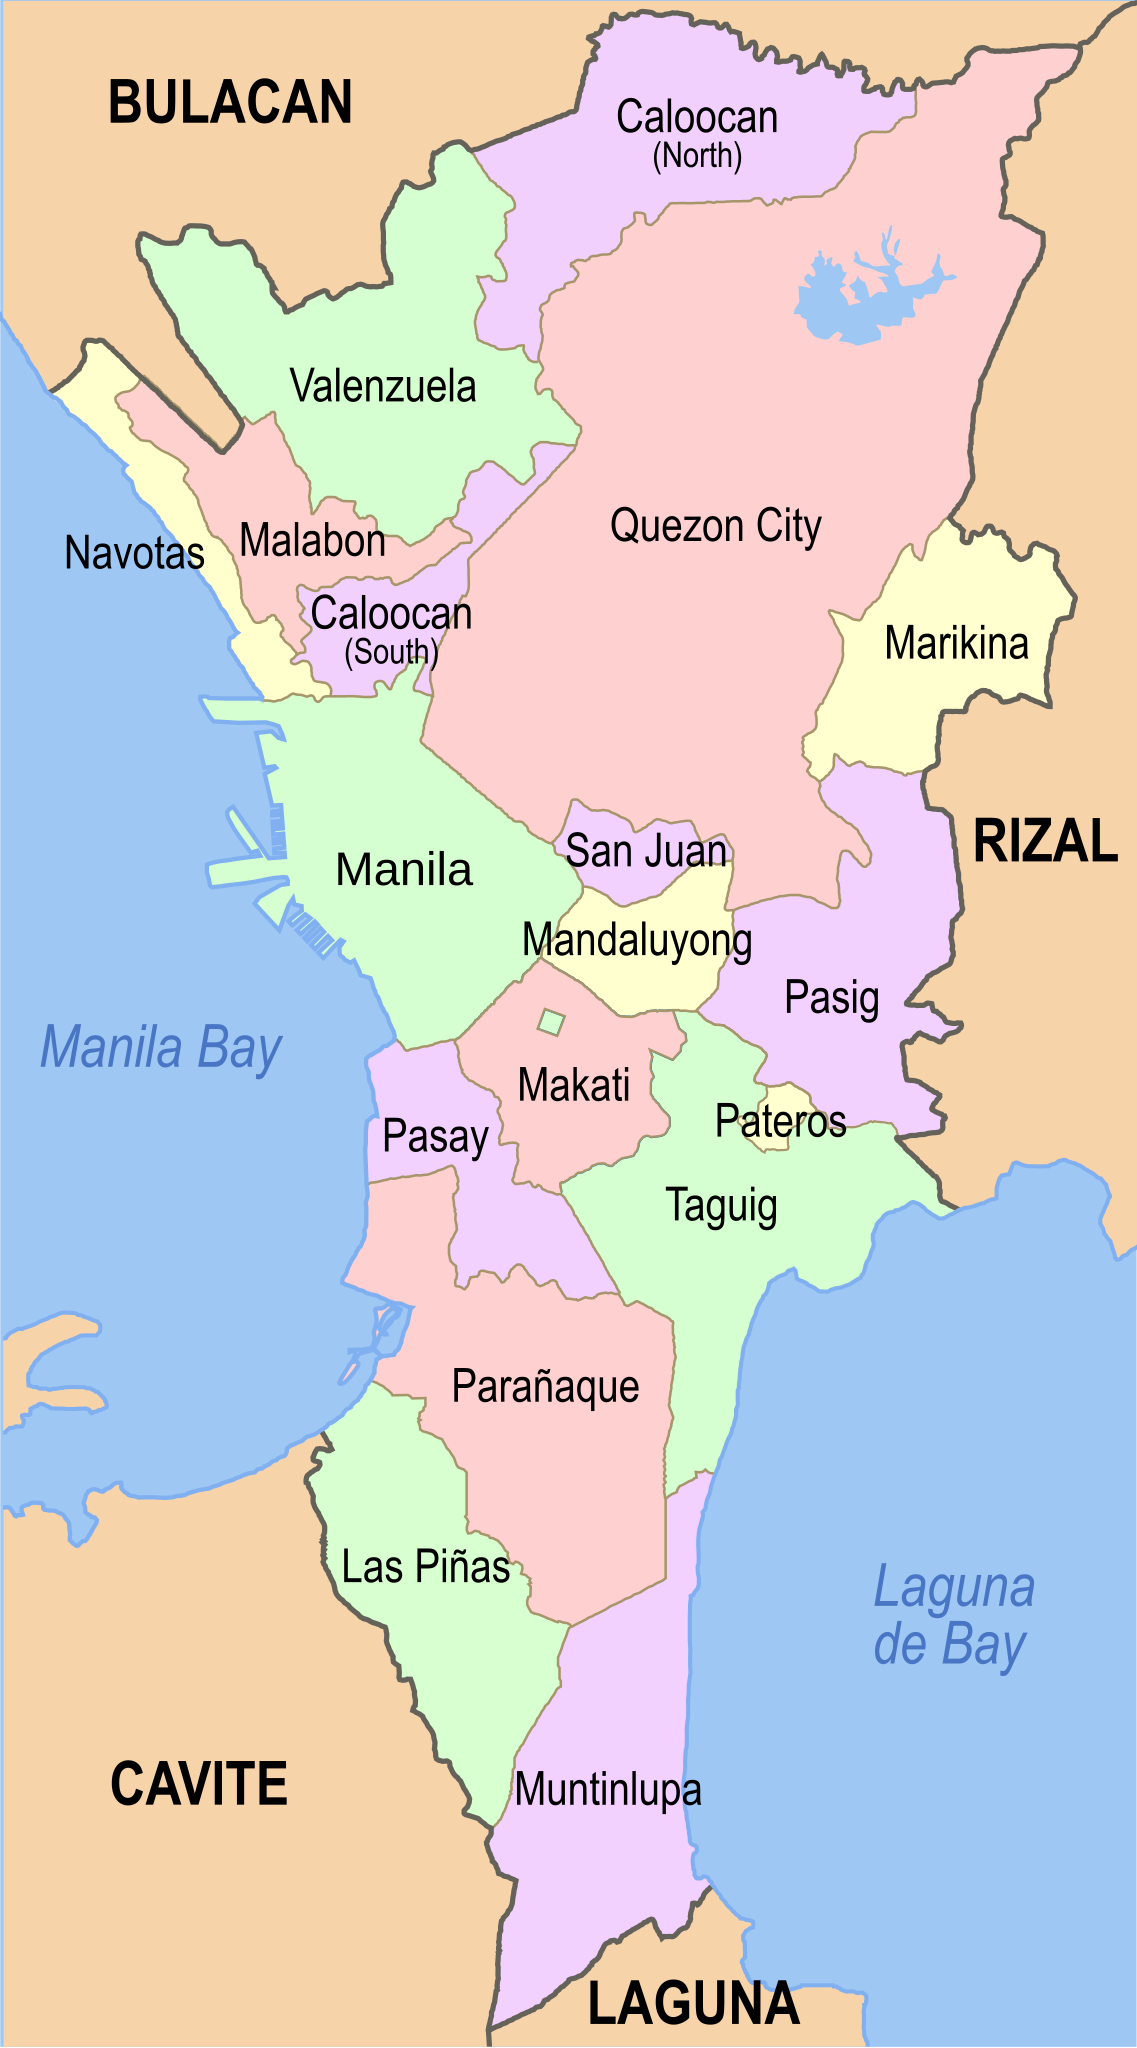
\includegraphics[width=10cm]{map-of-metro-manila}
		\caption{
			A map of Metro Manila.
			Created by Wikimedia user Philtro, and shared under a
			\href{https://creativecommons.org/licenses/by-sa/3.0/deed.en}{Creative Commons Attribution-Share Alike 3.0 Unported license}.
		}
		\label{fig:map-of-metro-manila}
	\end{figure}	
		
\section{Simulation Model}
	This study will use the latest version of the Regional Climate Model, RegCM5, which is described in detail by \textcite{Giorgi2023}.
	RegCM5 is a limited area model for long-term regional climate simulation.
	It is developed by the Abdus Salam International Centre for Theoretical Physics.
	The previous version, RegCM4, was released in 2012 (\cite{Giorgi2012}).
	
	\begin{table}	
		\caption{Configuration of the RegCM5 physics schemes.}
		\label{tab:physics-schemes}
		\centering
		\begin{tabular}{p{2 in} p{2.75 in}}
			\hline \hline
			Physics scheme & Configuration\\
			\hline
			Atmospheric radiation & Radiation scheme from the Community Climate Model version 3 (\cite{Kiehl1996}) \\
			Land surface model & Community Land Model version 4.5 (\cite{Oleson2013})\\
			Planetary boundary layer & Based on \textcite{Holtslag1990}\\
			Cumulus convection & Based on \textcite{Emanuel1991}\\
			Resolvable scale precipitation & Subgrid explicit moisture scheme (SUBEX) (\cite{Pal2000})\\
			\hline
		\end{tabular}		
	\end{table}

	This study will conduct simulations over two 20-year periods.
	The first simulation will be conducted from 2004 to 2023 to study the present.
	The results of this simulation will be compared to real meteorological data in order to determine the performance of the simulation.
	After the simulation has been evaluated to perform well, the second simulation will be run.
	The second simulation will be conducted from 2021 to 2040 to study the future.
	
	Table \ref{tab:physics-schemes} shows the physics schemes to be used in the study.
	These schemes, with the exception of the land surface model, will be used because they are the default schemes. 
	For the land surface model, the Community Land Model version 4.5 is chosen over the default, the Biosphere-Atmosphere Transfer Scheme. 
	The Community Land Model has a model for urban energy balance and climate, which the default model lacks.
	
\section{Simulation Evaluation}
	To determine the performance of the simulation, its results will be compared to real data from the Integrated Surface Database (ISD).
	The ISD is maintained by the United States National Oceanic and Atmospheric Administration, and is readily available on their website 
		(https://www.ncei.noaa.gov/products/land-based-station/integrated-surface-database).
	
	To evaluate the simulation, four performance statistics will be computed using equations \ref{eq:mean-bias} to \ref{eq:y-bar},
		where $y_i$ is the modeled value, $y_{i,\text{obs}}$ is the observed value, and $N$ is the number of data points (\cite{Bilang2022}).
	The mean bias (MB) is a measure of the model to overestimate or underestimate a variable, and is calculated by
	\begin{equation}
		\text{MB} =
			\frac{1}{N}
			\sum_{i=1}^{N}
			(y_i - y_{i,\text{obs}}).
			\label{eq:mean-bias}
	\end{equation}
	The root mean square error (RMSE) is similar to the MAE but more sensitive to large errors due to the squared term.
	It is calculated by
	\begin{equation}
		\text{RMSE} =
			\sqrt{
				\frac{
					\sum_{i=1}^{N}
					(y_i - y_{i,\text{obs}}) ^ 2
				}{N}
			}.
			\label{eq:root-mean-square-error}
	\end{equation}
	The mean absolute error (MAE) is used to measure the closeness of the modeled and observed values.
	It is calculated by
	\begin{equation}
		\text{MAE} =
			\frac{1}{N}
			\sum_{i=1}^{N} 
			|y_i - y_{i,\text{obs}}|. \label{eq:mean-absolute-error}
	\end{equation}
	Lastly, the index of agreement (IOA) shows how an error-free model predicts a variable.
	It is computed as
	\begin{equation}
		\text{IOA} =
			1 - 
			\frac{
				\sum_{i=1}^{N}
				(y_i - y_{i,\text{obs}}) ^ 2
			}{
				\sum_{i=1}^{N} (
					|y_i - \bar{y}| +
					|y_{i,\text{obs}} - \bar{y}|
				)^2
			}.
			\label{eq:index-of-agreement}
	\end{equation}
	where
	\begin{equation}
		\bar{y} = 
			\frac{1}{N}
			\sum_{i=1}^{N} y_{i,\text{obs}}
			\label{eq:y-bar}
	\end{equation}
	The threshold for these values to determine if the model is performing well are given in Table \ref{tab:performance-statistics-threshold}, as adapted from \textcite{Bilang2022}.

	\begin{table}	
		\caption{Recommended values of statistical tests for near-surface air temperature.}
		\label{tab:performance-statistics-threshold}
		\centering
		\begin{tabular}{l l}
			\hline \hline
			Statistical parameter & Criteria\\
			\hline
			MB & $\leq \pm \qty{2.0}{\degreeCelsius}$ \\
			RMSE & $\leq \qty{3.5}{\degreeCelsius}$\\
			MAE & $\leq \pm \qty{2.0}{\degreeCelsius}$\\
			IOA	& $\geq \num{0.8}$\\
			\hline
		\end{tabular}		
	\end{table}

\section{Data Graphing and Analysis}
	The results of the simulations will be graphed.
	Data for the near-surface air temperature will be graphed as a function of time.
	This is to visually see the trend of the air temperature as time progresses.
	For the simulation of the present time, the graph of the simulation results will be overlayed on the graph of the observed data from the ISD.
	This is to visually compare the performance of the simulation with actual data.
	
	The results of the simulations will also be statistically analyzed.
	Descriptive statistics for the near-surface air temperature, such as the mean, maximum, and minimum temperature, will be computed.
	A linear regression will also be applied to see the trend at which temperature changes as time progresses.